\documentclass[11pt,spanish]{beamer}
\usetheme{CambridgeUS}					% Tema de las diapositivas
\usepackage[utf8]{inputenc}				% Idioma
\usepackage{amsmath,amsfonts,amssymb}   % Caracteres propios de las matematicas
\usepackage{graphicx, epstopdf}			% Para insertar imagenes
\usepackage{booktabs}					% Insertar tablas con formatos bonitos
\usepackage{tikz}
\usetikzlibrary{shapes,arrows,calc,positioning}
\usepackage{color}	
\newcommand{\red}{\textcolor{red}}
\newcommand{\white}{\textcolor{white}}
\providecommand{\abs}[1]{\lvert#1\rvert} 	  % Valor absoluto
\providecommand{\norm}[1]{\lVert#1\rVert}	  % Norma

\author{Felipe Galarce Marin}
\title{Proyecto de Ingeniería Civil - Semestre I}
\setbeamercovered{transparent} 
%\setbeamertemplate{navigation symbols}{} 
%\logo{} 
%\institute{} 
%\date{} 
%\subject{} 
\begin{document}

\frame{\frametitle{CIV661: Proyecto de Ingeniería Civil - Semestre I}
\begin{center}
\includegraphics[scale=0.3]{fig/logo}\\
\textbf{Modelación y Simulación Computacional de un Medio Fibroso: Aplicación a la Estimación de Parámetros en Tejidos Cardíacos}
\end{center}
\vspace{0.2in}
\begin{center}
Felipe A. Galarce Marin \\
\vspace{0.2in}
\begin{small}
Profesor Guía: Joaquín Mura\\
Profesor Co-referente: Cristobal Bertoglio \\
Pontificia Universidad Católica de Valparaíso
\end{small}
\end{center}
}


\begin{frame}{Introducción}
\begin{itemize}
\item[-] Fibrosis \pause $\rightarrow$ Fibrilación Ventricular \pause $\rightarrow$ Paro Cardíaco (sudden cardiac arrest) \pause
\item[-] Fibrosis \pause $\rightarrow$ Propagación del Potencial Eléctrico en el tejido cardíaco \cite{TenTusscher2007Europace}
\begin{figure}
\includegraphics[height = 4 cm]{fig/intro1}
\end{figure}
\end{itemize}
\pause
Idea: estudiar los patrones de difusión del potencial electrico puede permitír, eventualmente, saber acerca de la existencia y tipología de tejidos fibrosos
\end{frame}

\begin{frame}{Anatomía}
\begin{figure}[H] % esquema corazón
\centering
\includegraphics[height = 6 cm]{fig/fundamentals-corazon}
\caption{diagrama esquemático de la anatomía del corazón. Fuente \cite{texas_inst} } \label{corazon}
\end{figure}
\end{frame}


\begin{frame}{Histología}
\begin{figure}[H]
\centering
\includegraphics[scale=.35]{fig/fundamentals-myocites}
\includegraphics[scale=.6]{fig/fundamentals-gap_junctions} 
\caption{celula cardíaca muscular y \textsl{gap junctions}.} 
\end{figure}
\end{frame}

\begin{frame}{Histología}
\begin{figure}[H]
\centering
\includegraphics[height = 4.5 cm]{fig/fundamentals-direccionmiocitos}
\caption{heart fiber orientation. Fuente: \cite{shearstrain-fiberorientation}} \label{orientacionmiocitos}
\end{figure}
\pause
Anisotropía (ortotropía):
\begin{equation}
D_h = d_1 \hat{f} \otimes \hat{f} + d_2 \hat{c} \otimes \hat{c}
\end{equation}
\end{frame}

\begin{frame}{Electrofisología: Potencial de Acción}
\begin{figure}[H]
\centering
\def\svgwidth{9 cm}
\input{fig/fundamentals-action_potential.pdf_tex}
\caption{squematic plot of a cardiac action potential with its phases. Fuente: \cite{action-potential-figure}} \label{action-potential}
\end{figure}
\end{frame}

\begin{frame}{Electrofisología}
\begin{figure}[H] % esquema conducción de corriente en el corazón
\centering
\includegraphics[height = 6 cm]{fig/fundamentals-sistema_de_conduccion}
\caption{esquema de la conducción del potencial electrico en el tejido cardíaco. Fuente \cite{electrofis}} \label{corazon_conduccion}
\end{figure}
\end{frame}

\begin{frame}{Fibrosis}

\begin{itemize}
\item Fibroblastos \pause $\rightarrow$ Colágeno \pause $\rightarrow$ Fibrosis \pause
\item Tipos de Fibrosis (según dispersión): stringy Fibrosis, \pause patchy Fibrosis \pause y diffuse Fibrosis,.
\end{itemize}

\begin{figure}[H]
\centering
\includegraphics[width = 3 cm]{fig/fundamentals-fib-stringy}
\includegraphics[width = 3 cm]{fig/fundamentals-fib-patchy} 
\includegraphics[width = 3 cm]{fig/fundamentals-fib-diffuse} 
\caption{diferentes tipos de fibrosis.}
\end{figure}

\end{frame}

\begin{frame}
\begin{figure}[H]
\includegraphics[width= 8 cm]{fig/fundamentals-fib-midvsdensity}
\caption{gráfico del MID (mean increase delay) v/s densidad para los distintos tipos de fibrosis (patchy, $*$; stringy, $\blacktriangle$; or diffuse, $\bullet$) . From \cite{Kawara2001Circ}}. \label{fig:midvsdensity}
\end{figure}
\end{frame}

\begin{frame}
\begin{center}
\Huge Modelación
\end{center}
\end{frame}

\begin{frame}{Modelación del Arreglo de Tejido Cardíaco}
\begin{itemize}
\item Modelo bi-dominio: 
\begin{itemize}
\item Alto costo computacional
\item Usualmente mal condicionado \cite{colli_franzone}. (\red{?})
\item Mas realista que modelo mono-dominio (considera potencial intra y extracelular y \textsl{gating variables}).
\end{itemize}
\pause
\item Modelo mono-dominio:
\begin{itemize}
\item Bajo costo computacional (en relación al modelo bi-dominio).
\item Considera un potencial medio.
\end{itemize}
\item Ambos Fenomenológicos: no se considera micro-estructura, como la existencia de \textsl{gap-junctions}.
\end{itemize}
\end{frame}


\begin{frame}{Modelo Bi-Dominio}
\textbf{PP-formulation:} 

\begin{equation}
\arraycolsep=1.4pt\def\arraystretch{2.2}
\left\lbrace
\begin{array}{lr}
c_m \dfrac{\partial v}{\partial t} - div(D_i \nabla u_i) + I_{ion}(v,w,z) = I_{i}^s & \text{ in } \Omega \times (0,T) \\
-c_m \dfrac{\partial v}{\partial t } - div(D_e \nabla u_e) - I_{ion}(v,w,z) = I_e^s & \text{ in }\Omega \times (0,T) \\
\dfrac{\partial z}{\partial t} - F(v,w) = 0 & \text{ in }\Omega \times (0,T) \\
\dfrac{\partial z}{\partial t } - G(v,w,z) = 0  & \text{ in }\Omega \times (0,T) \\
D_{i,e}  \nabla u_{i,e} \cdot \hat{n} = 0 & \text{ in } \Gamma_N \times (0,T) \\
+ \text{ Dirichlet Conditions }
\end{array}
\right.  \label{eq:BDM}
\end{equation}
\end{frame}

\begin{frame}{Modelo Mono-Dominio}

Algunas definiciones:
\begin{itemize}
\item El dominio $\Omega \in \mathbb{R}^d$ ($d = 2,3$).
\item El potencial eléctrico $\phi: \Omega \times \mathbb{R^+}$.
\item El vector de variables internas que regula la recuperación de la celula (i.e., el potencial de acción) $\vec{r}: \Omega \times \mathbb{R}^+ \rightarrow \mathbb{R}^m$, donde m es la cantidad de parámetros usados para modelar los procesos de la membrana celular.
\item La capacitancia de la membrana $C_{\phi} \in \mathbb{R}$.
\item El tensor de difusión $D \in \mathbb{R}^{d \times d}$.
\item El tensor $C_r \in \mathbb{R}^{m \times m}$.
\end{itemize}
\end{frame}

\begin{frame}{Modelo Mono-Dominio}
\begin{itemize}
\item Si los medios tienen el mismo \textsl{anisotropy ratio} (lo cual es falso), entonces las ecuaciones de bi-donimio se reducen a:
\end{itemize}
\begin{equation}
\arraycolsep=1.4pt\def\arraystretch{2.2}
\left\lbrace
\begin{array}{lr}
\dfrac{\partial \phi}{ \partial t} - div(D \nabla \phi) = f^{\phi}(\phi, \vec{r}) \\
\dfrac{\partial r}{\partial t} =  f^{r}(\phi, \vec{r})\\
\text{ + boundary conditions }
\end{array}
\right.  \label{eq:MDE}
\end{equation}
Nuevamente, la elección de $f^{\phi}$ y $f^{r}$ depende del modelo a utilizar para describir la actividad eléctrica de la membrana celular.
\end{frame}

\begin{frame}{Modelación de la Actividad Eléctrica de la Membrana Celular}

\begin{itemize}
\item Hodkin-Huxley Model
\item The Beeler-Reuter Model
\item The Luo Rudy I Model (LR1) \pause
\item Modelos Simplificados/Reducidos:
\begin{itemize}
\item Aliev-Panfilov Model
\item Mitchel-Schaeffer Model \pause
\item \red{FitzHugh-Nagumo Model}
\end{itemize}
\end{itemize}
\begin{figure}[H]
\centering
\includegraphics[height = 3.1 cm]{fig/membrana_1}
\end{figure}
\end{frame}

\begin{frame}{Modelo Mono-Dominio +FHN}

Modelo a usar para la reacción-difusión del potencial eléctrico en el tejido cardíaco:

\begin{equation}
\arraycolsep=1.4pt\def\arraystretch{2.2}
\left\lbrace
\begin{array}{lr}
\dfrac{\partial \phi}{ \partial t} - div(D \nabla \phi) = c_1 \phi (\phi - \alpha)(1 - \phi) - c_2 r \\ 
\dfrac{\partial r}{\partial t} = c_2 (\phi - rd)\\
\text{ + condiciones de borde }
\end{array}
\right. \label{modelo_final}
\end{equation}
\end{frame}

\begin{frame}{Método}
\begin{itemize}
\item Resolver MDE+FHN sobre un medio con propiedades de difusión variables \pause $\rightarrow$ Colageno
\item \pause Apagar celulas.
\end{itemize}
\centering
\includegraphics[height = 4 cm]{fig/theorem_verification_r2-laminations} 

\pause
\textbf{¡Alto costo computacional!}

\end{frame}

\begin{frame}
\begin{center}
\Huge Método Multiescala
\end{center}
\end{frame}

\begin{frame}
\begin{itemize}
\item Resolver ecuaciones (\label{modelo_final}) sobre un medio con propiedades de difusión variables $\rightarrow$ Colageno
\item  Apagar celulas.
\end{itemize}
\centering
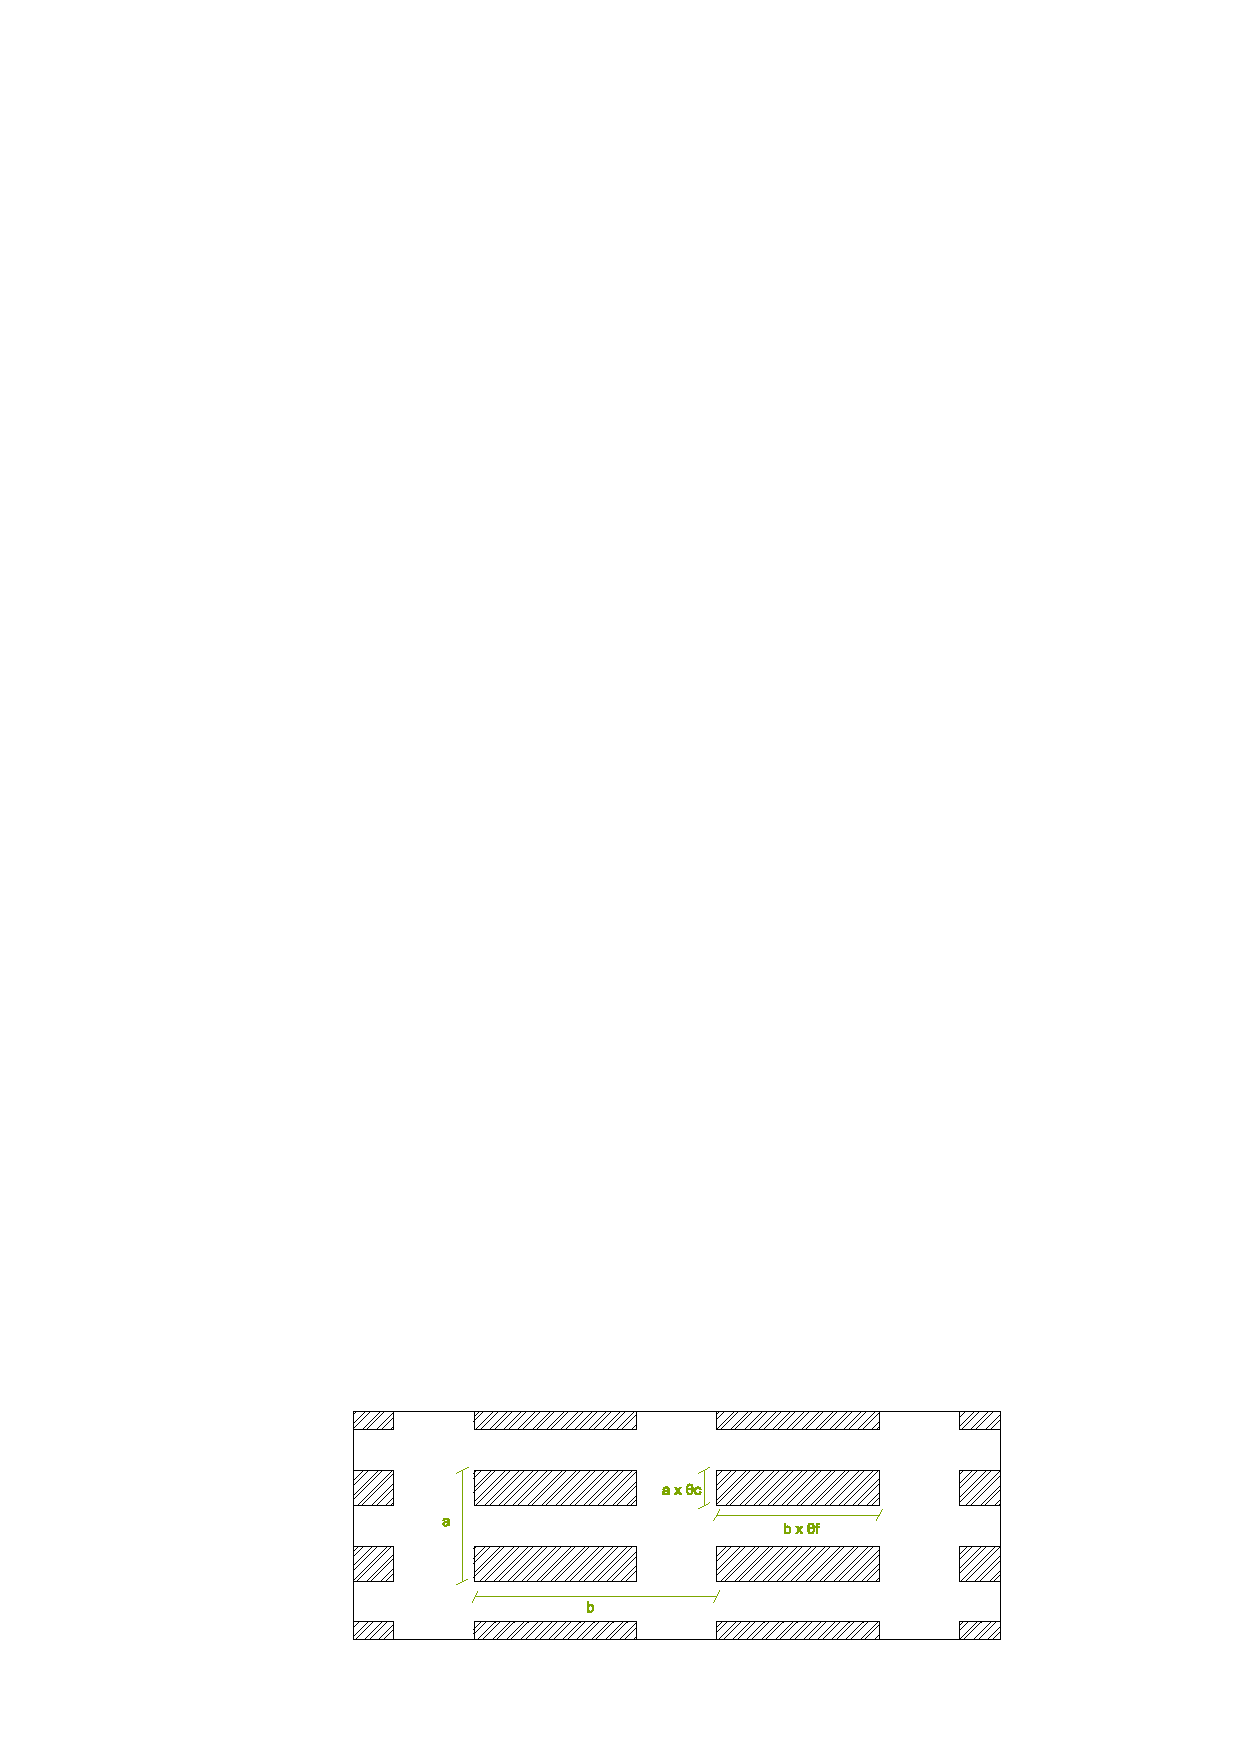
\includegraphics[height = 4 cm]{fig/theorem_verification_r2-geometry_convention.png} \\
\textbf{¡Alto costo computacional!}

\end{frame}

\begin{frame}{Método Multiescala}

\pause
\begin{itemize}
\item Homogeneización por laminaciones (rango 2)\pause
\item Tensor de difusión efectivo \pause
\item La homogeneización del modelo MDE+FHN no es (aún) posible. \pause
\item Sin embargo, si se puede demostrar que la solución de el siguiente modelo (ecuación de difusión!):
\end{itemize}

\begin{equation}
\left\lbrace
\begin{array}{c} 
-div( D \nabla \phi ) = f \label{difusion} \\
\text{ + condiciones de borde}
\end{array}
\right.
\end{equation}

\noindent donde $\hat{n}$ es un vector unitario y normal a la frontera del dominio, $f$ es una fuente interna y $D$ se define como:

\begin{equation*}
D = \left\lbrace \begin{array}{lr}

D_1 \text{ on } \Omega_1 \subset \Omega \\
D_2 \text{ on } \Omega_2 \subset \Omega & \rightarrow \text{ ``Colágeno'' }

\end{array} \right.
\end{equation*}
\noindent donde $\Omega_1 \cap \Omega_2 = \oslash$ y $\Omega_1 \cup \Omega_2 = \Omega$.
\end{frame}

\begin{frame}{Homogeneización}

...converge a la solución de:

\begin{equation}
\left\lbrace
\begin{array}{c} 
-div(D^{eff} \nabla \phi_h )= f \label{difusion_eff}\\
\text{ + condiciones de borde}
\end{array}
\right.
\end{equation}

conforme el tamaño de $\Omega_2$ tiende 0. Al tensor $D^{eff}$ se le llamará \textsl{tensor efectivo}, y viene dado por:

\begin{equation*}
D_{eff} = 
(1 - \theta_f)D_h + \theta_f D_{eff}' - \frac{\theta_f (1 - \theta_f)(D_{eff}' - D_h)e_2 \otimes (D_{eff}' - D_h)^T e_2}{(1 - \theta_f)D_{eff}' e_2 \cdot e_2 + \theta_f D_h e_2 \cdot e_2 }
\end{equation*}

en donde,

\begin{equation*}
D_{eff}'=
(1 - \theta_c)D_h + \theta_c D_{col} - \frac{\theta_c (1 - \theta_c)(D_{col} - D_{h})e_1 \otimes (D_{col} - D_{h})^T e_1}{(1 - \theta_c)D_{col} e_1 \cdot e_1 + \theta_c D_{h} e_1 \cdot e_1 }
\end{equation*}
\end{frame}

\begin{frame}{Verificación Numérica del Teorema}

Ejemplo Numérico \#1:

\begin{itemize}
\item Caso estático.
\item Laminaciones de rango 1.
\item $\Omega = [0,0]\times[10 \text{ mm}, 10 \text{ mm}]$.
\item Tensor de difusión del medio:
\begin{equation*}
D_1 = d_1 \left[ \begin{array}{cc}
1 & 0 \\
0 & 1
\end{array} \right] 
\end{equation*}
donde  $d_1 = 0.1 [mm^2/s]$.

\item Tensor de difusión de laminaciones:
\begin{equation*}
D_2 = \alpha D_1
\end{equation*}
$\alpha \in [0,1]$.

\item Dirección de laminación: $e_1 = (1,0,0)$
\end{itemize}
\end{frame}

\begin{frame}{Verificación Numérica del Teorema}

\begin{itemize}

\item Condiciones de borde:

\begin{equation*}
\left\lbrace
\begin{array}{c}
D \nabla \phi \cdot \hat{n} = 0 \text{ on right and up boundaries} \\
\phi = \dfrac{ e^{\frac{-(x - \mu)^2}{2 \sigma^2}}}{2 \pi \sqrt{2 \pi}} \text{ on bottom boundary} \\
\phi = \dfrac{ e^{\frac{-(y - \mu)^2}{2 \sigma^2}}}{2 \pi \sqrt{2 \pi}} \text{ on left boundary}
\end{array}
\right. \label{eq:border_conditions_r1}
\end{equation*}

\item Forma Variacional Débil: 

\begin{equation}
V = \{ v \in H^1(\Omega): v = 0 ~\text{on}~ \Gamma_D \}
\end{equation}

\begin{equation*}
\int_\Omega (D^{eff} \nabla \phi_h) \nabla v d \Omega = \int_\Omega fv d\Omega  + \int_{\Gamma_N} g v ds ~~ \forall v \in \hat{V}_h \subset \hat{V}
\end{equation*}
\end{itemize}
\end{frame}


\begin{frame}
\begin{figure}[H]
\centering
\includegraphics[height = 5 cm]{fig/theorem_verification_r1-mesh_nh} 
\caption{zoom of mesh used for non-homogenized problems}
\end{figure}
\end{frame}

\begin{frame}{Verificación Numérica del Teorema}
\begin{figure}[H]
\centering
\includegraphics[height = 4 cm]{fig/theorem_verification_r1-malla_gruesa}
\caption{mesh used for homogenized problems}\label{fig:verification-malla_gruesa}
\end{figure}
\end{frame}

\begin{frame}{Verificación Numérica del Teorema}
\begin{figure}[H]
\centering
\includegraphics[height = 4 cm]{fig/theorem_verification_r1-beta001}
\caption{solution of the problems \ref{difusion} and \ref{difusion_eff} for $\beta = 0.01$.} 
\end{figure}
\end{frame}

\begin{frame}{Verificación Numérica del Teorema}
\begin{figure}[H]
\centering
\includegraphics[height = 4 cm]{fig/theorem_verification_r1-beta10_-5}
\caption{solution of the problems \ref{difusion} (left) and \ref{difusion_eff} (right) for $\beta = 10^{-5}$.} 
\end{figure}
\end{frame}

\begin{frame}{Verificación Numérica del Teorema}
\begin{figure}[H]
\centering
\includegraphics[height = 4 cm]{fig/theorem_verification_r1-beta10_5}
\caption{solution of the problems \ref{difusion} (left) and \ref{difusion_eff} (right) for $\beta = 10^{5}$. Error $= 0.088$} \label{fig:verification-beta10e+5}
\end{figure}
\end{frame}

\begin{frame}{Verificación Numérica del Teorema}

Como medida para estimar el error se usó la norma L2, esto es:

\begin{equation}
\text{error} = \frac{\norm{\phi - \phi_h}_{L2}}{\norm{\phi}_{L2}} = \frac{\int_{\Omega} (\phi - \phi_h)^2 d\Omega}{\int_{\Omega} \phi^2 d \Omega}
\end{equation}

\begin{figure}[H]
\centering
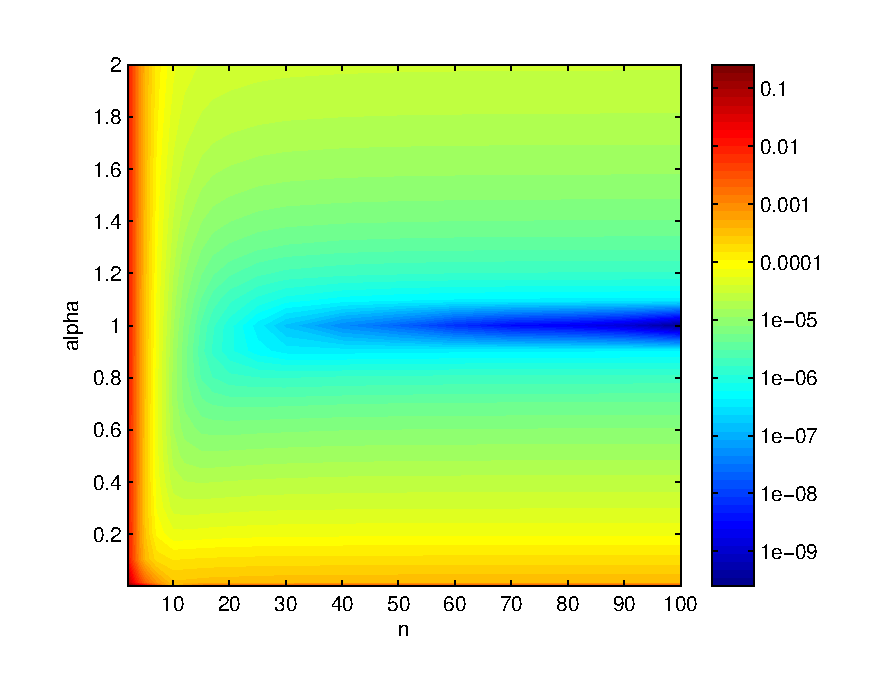
\includegraphics[height = 5 cm]{fig/theorem_verification_r1-error_l2}
\caption{Error en norma L2 para distintos valores $\alpha$ y $n$ (escala logarítmica en $\phi$).}
\end{figure}
\end{frame}

\begin{frame}{Verificación Numérica del Teorema}
Ejemplo Numérico \#2: 
\begin{itemize}
\item Caso dinámico.
\item Laminaciones de Rango 2.
\item Configuración:
\begin{table}[H]
\centering
\label{tab:geometric_setup_diff_r2}
\begin{tabular}{@{}ccccccccc@{}}
\toprule
       & \# DOF's & a {[}mm{]} & b {[}mm{]} & $\theta_c$ & $\theta_f$ & $\beta$   & $\gamma$ & $\Omega$ \\ \midrule
	   & 232324   & 0.1        & 1          & 0.4        & 0.5        & $10^{-5}$ & 5        & $6 \times 6 [mm^2]$ \\ \bottomrule
\end{tabular}
\end{table}
\end{itemize}
\begin{equation}
\arraycolsep=1.4pt\def\arraystretch{2.2}
\left\lbrace
\begin{array}{lr}
\frac{\partial \phi}{ \partial t} - div(D^{eff} \nabla \phi) = f \\
\phi = \overline{\phi} \text{ on } \Gamma_D \\
D \nabla \phi \cdot  \hat{n} = g \text{ on } \Gamma_N \\
\end{array}
\right.
\end{equation}
\end{frame}

\begin{frame}
\begin{itemize}
\item Condiciones de borde Neumann.
\item Forma Variacional Débil Discretizada en el Tiempo (Backward Euler):
\begin{equation*}
\arraycolsep=1.4pt\def\arraystretch{2.2}
\left\lbrace
\begin{array}{lr}
a_k(\phi_k, v) = \int_{\Omega} \phi_k v + \Delta t (D \nabla \phi_k) \nabla v  d \Omega \\
L_k(v) = \Delta t\int_{\Omega} f_k  v d \Omega + \int_{\Omega} \phi_{k-1} v d \Omega + \Delta t  \int_{\Gamma_N} g v ds
\end{array}
\right. 
\end{equation*}
\end{itemize}
\end{frame}

\begin{frame}
\begin{figure}[H]
\centering
\includegraphics[height = 0.9 cm]{fig/theorem_verification_r2_exp2_colorbar}
\end{figure}
\begin{figure}[H]
\centering
\includegraphics[height = 5 cm]{fig/theorem_verification_r2_exp2_5ms}
\caption{5 [ms]}
\end{figure}
\end{frame}

\begin{frame}
\begin{figure}[H]
\centering
\includegraphics[height = 0.9 cm]{fig/theorem_verification_r2_exp2_colorbar}
\end{figure}
\begin{figure}[H]
\centering
\includegraphics[height = 5 cm]{fig/theorem_verification_r2_exp2_70ms}
\caption{70 [ms]}
\end{figure}
\end{frame}

\begin{frame}
\begin{figure}[H]
\centering
\includegraphics[height = 0.9 cm]{fig/theorem_verification_r2_exp2_colorbar}
\end{figure}
\begin{figure}[H]
\centering
\includegraphics[height = 5 cm]{fig/theorem_verification_r2_exp2_258ms}
\caption{258 [ms]}
\end{figure}
\end{frame}

\begin{frame}
\begin{figure}[H]
\centering
\includegraphics[height = 0.9 cm]{fig/theorem_verification_r2_exp2_colorbar}
\end{figure}
\begin{figure}[H]
\centering
\includegraphics[height = 5 cm]{fig/theorem_verification_r2_exp2_400ms}
\caption{400 [ms]}
\end{figure}
\end{frame}

\begin{frame}
\begin{figure}[H]
\centering
\includegraphics[height = 0.9 cm]{fig/theorem_verification_r2_exp2_colorbar}
\end{figure}
\begin{figure}[H]
\centering
\includegraphics[height = 5 cm]{fig/theorem_verification_r2_exp2_800ms}
\caption{800 [ms]}
\end{figure}
\end{frame}

\begin{frame}
\begin{figure}[H]
\centering
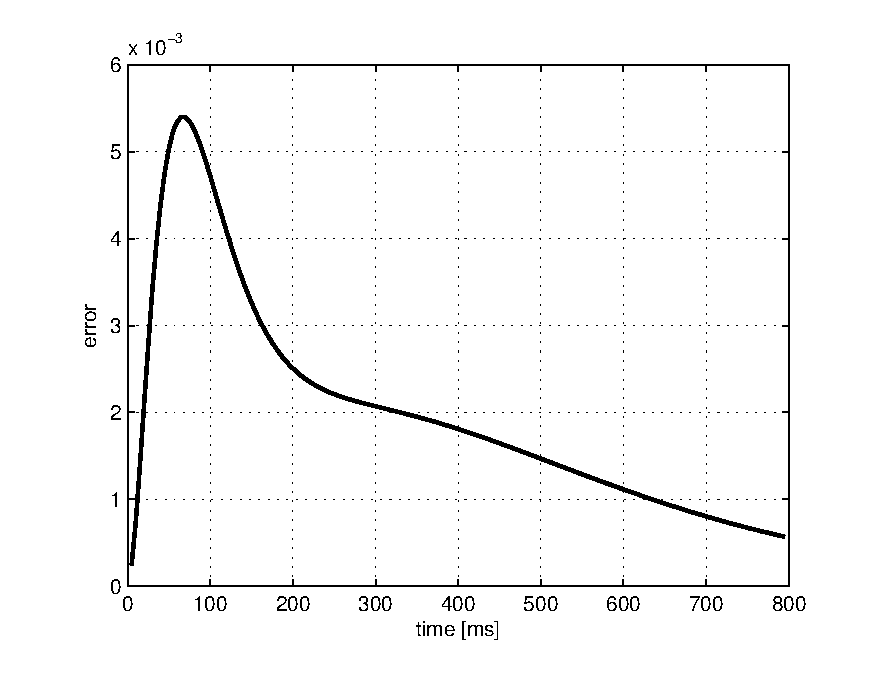
\includegraphics[height = 6 cm]{fig/theorem_verification_r2_exp2_error}
\caption{error v/s time for experiment \# 2}
\end{figure}
\end{frame}

\begin{frame}
\begin{center}
\Huge Modelación de fibrosis difusa mediante modelo efectivo.
\end{center}
\end{frame}

\begin{frame}{Surrogated Model}
\begin{itemize}
\item Con el teorema ya verificado, se procede a utilizar el mismo tensor $D^{eff}$ en las ecuaciones de monodominio, con la esperanza de que el error entre la solución homogeneizada y la exacta sea pequeño \\
\begin{center}
\pause $\rightarrow$ \textbf{``Surrogated Model''}
\end{center} 
\end{itemize}
\end{frame}

\begin{frame}{Análisis de Estabilidad del modelo MDE+FHN}
``Energía'' total del sistema continuo:
\begin{equation*}
E = \red{c_1 (1 + \alpha) \phi^3} - c_1 (\alpha \phi^2 +  \phi^4) -c_2 d r^2 \label{eq:total_energy}
\end{equation*}
\pause
``Energía'' total del sistema discretizado en el tiempo (notar discretización ``conveniente''): 

\begin{equation*}
\arraycolsep=1.4pt\def\arraystretch{2.2}
\begin{array}{lr}
\overline{E} = & c_2 \phi^{n + \beta} r^{n + \theta} - c_2 d (r^{n + \theta})^2 
 - \red{(\theta - \frac{1}{2}) \frac{1}{\Delta t} (r^{n+1} - r^n)^2}  \\
& + \red{ c_1 (1 + \alpha) \phi^n (\phi^{n + \beta})^2} - c_1 \alpha (\phi^{n + \beta})^{2}
- c_1 (\phi^n)^2 (\phi^{n + \beta})^2 \\
& - c_2 r^{n + \theta} v^{n + \beta}
- \red{(\beta - \frac{1}{2}) \frac{1}{\Delta t} (\phi^{n+1} - \phi^n)^2 }
\end{array}
\end{equation*}
\end{frame}

\begin{frame}{Discretización en el Tiempo}
Se escoge finalmente el siguiente esquema (\red{por qué?}):

\begin{equation*}
\arraycolsep=1.4pt\def\arraystretch{2.2}
\begin{array}{llr}
\dfrac{r^{n+1} - r^n}{\Delta t} = c_2 \phi^n - c_2 d r^{n+1} \\
\dfrac{\phi^{n+1} - \phi^n}{\Delta t} = c_1 (1 + \alpha) (\phi^n)^2 - c_1 \alpha \phi^{n+1} - c_1 (\phi^n)^3 + div(D \nabla \phi^{n+1})
\end{array}
\end{equation*}

\begin{itemize}
\pause
\item Términos lineales implícitos.\pause
\item Términos no-lineales explícitos.  \pause
\item Difusión implícita. \pause
\end{itemize}
\textbf{Observación:} problema desacoplado!
\end{frame}

\begin{frame}{Problema Final}

Encontrar $r^{n+1}$ tal que:

\begin{equation*}
r^{n+1} = r^n + \Delta t c_2 (\phi^n - r^{n+1} d)
\end{equation*}

para luego resolver $a_{n + 1} (\phi^{n + 1}, v) = L(v)$, donde:

\begin{equation*}
a_{n+1} (\phi^{n + 1}, v) = \int_{\Omega} (1 + \Delta t c_1 \alpha) \phi^{n+1} v d \Omega + \Delta t \int_{\Omega} D \nabla \phi^{n+1} \nabla v d \Omega \label{eq:esquema_definitivo}
\end{equation*}
\begin{equation*}
L_{n+1}(v) = \int_{\Omega} \phi^n v d \Omega + \Delta t \int_\Omega \{ c_1(1 + \alpha)(\phi^n)^2 - c_1 (\phi^n)^3 - c_2 r^{n+1} \} v d \Omega + \Delta t \int_{\Gamma_N} g  v ds 
\end{equation*}
\end{frame}

\begin{frame}{Ejemplos Numéricos}
Ejemplo numérico \# 2.5:
\begin{itemize}
\item Dominio: una sola célula (no hay difusión).
\item Discretización temporal implícita.
\item Problema acoplado.
\item Método de Quasi-Newton.
\end{itemize}
\end{frame}

\begin{frame}
\begin{figure}[H]
\centering 
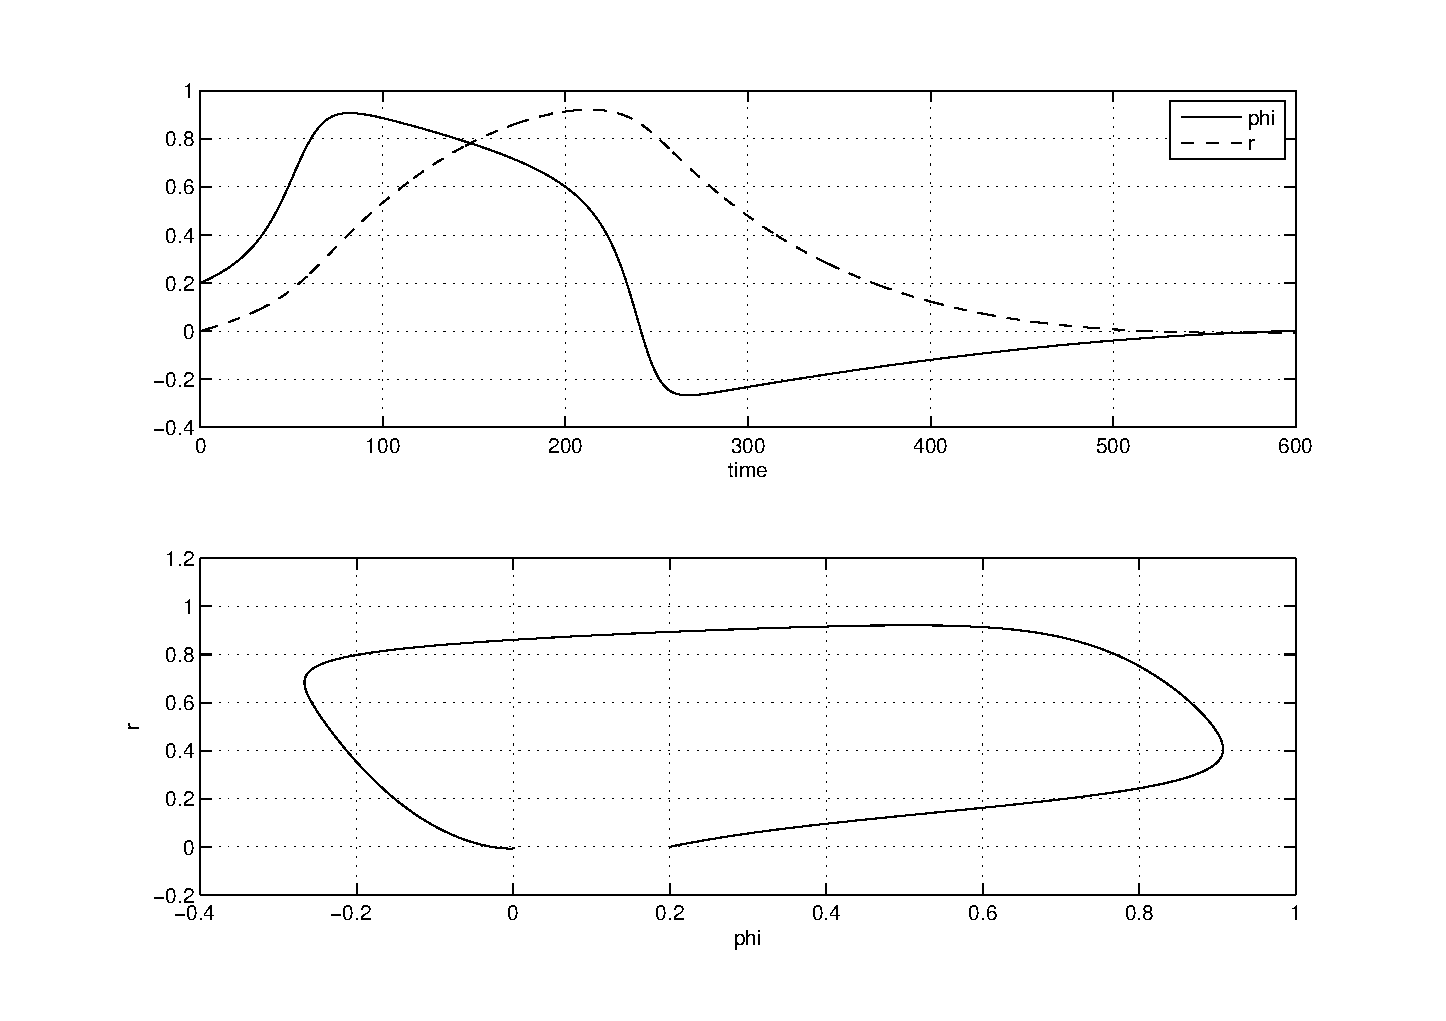
\includegraphics[height = 8.5 cm]{fig/reaction_term-FHN_implicit}
\caption{Numerical solution of the FitzHugh-Namuno equations using $c_1 = 0.175$, $c_2 = 0.03$, $\Delta t = 18 [ms]$, $d = 0.55$ and $\alpha = 0.08$.}
\end{figure}
\end{frame}

\begin{frame}{Ejemplos Numéricos}
Ejemplo numérico \# 3:

\begin{itemize}
\item Dominio: $20 \times 20 [mm^2]$
\begin{table}[H]
\centering
\begin{tabular}{@{}cccccccc@{}}
\toprule
 \# DOF's & a {[}mm{]} & b {[}mm{]} & $\theta_c$ & $\theta_f$ & $\beta$   & $\gamma$ & $\Delta t$ [ms]\\ \midrule
 \red{328854}   & 0.1        & 1          & 0.5        & 0.5        & $10^{-5}$     & 5   & 10     \\ \bottomrule
\end{tabular}
\caption{setup for experiment.} 
\end{table}
\item Grados de libertad para problema homogeneizado: \red{841}.
\end{itemize}
\end{frame}


\begin{frame}
\begin{figure}[H]
\centering
\includegraphics[height = 0.9 cm]{fig/numerical_example_MDE_exp3_colourbar}
\end{figure}
\begin{figure}[H]
\centering
\includegraphics[height = 5 cm]{fig/numerical_example_MDE_exp3_20ms}
\caption{20 [ms]}
\end{figure}
\end{frame}

\begin{frame}
\begin{figure}[H]
\centering
\includegraphics[height = 0.9 cm]{fig/numerical_example_MDE_exp3_colourbar}
\end{figure}
\begin{figure}[H]
\centering
\includegraphics[height = 5 cm]{fig/numerical_example_MDE_exp3_200ms}
\caption{200 [ms]}
\end{figure}
\end{frame}

\begin{frame}
\begin{figure}[H]
\centering
\includegraphics[height = 0.9 cm]{fig/numerical_example_MDE_exp3_colourbar}
\end{figure}
\begin{figure}[H]
\centering
\includegraphics[height = 5 cm]{fig/numerical_example_MDE_exp3_600ms}
\caption{600 [ms]}
\end{figure}
\end{frame}

\begin{frame}
\begin{figure}[H]
\centering
\includegraphics[height = 0.9 cm]{fig/numerical_example_MDE_exp3_colourbar}
\end{figure}
\begin{figure}[H]
\centering
\includegraphics[height = 5 cm]{fig/numerical_example_MDE_exp3_1000ms}
\caption{1000 [ms]}
\end{figure}
\end{frame}

\begin{frame}

Métodos de resolución de los sistemas lineales:

\begin{itemize}
\item Problema Exacto \pause $\rightarrow$ Preacondicionador (AMG HYPRE) + Gradiente Conjugado 
\item Problema Homogeneizado \pause $\rightarrow$ Eliminación Gaussiana.
\end{itemize}

Además, en ambos casos, el proceso de ensamblaje se realizó una sola vez antes de comenzar las iteraciones en el tiempo.
\pause
\begin{figure}[H]
\centering
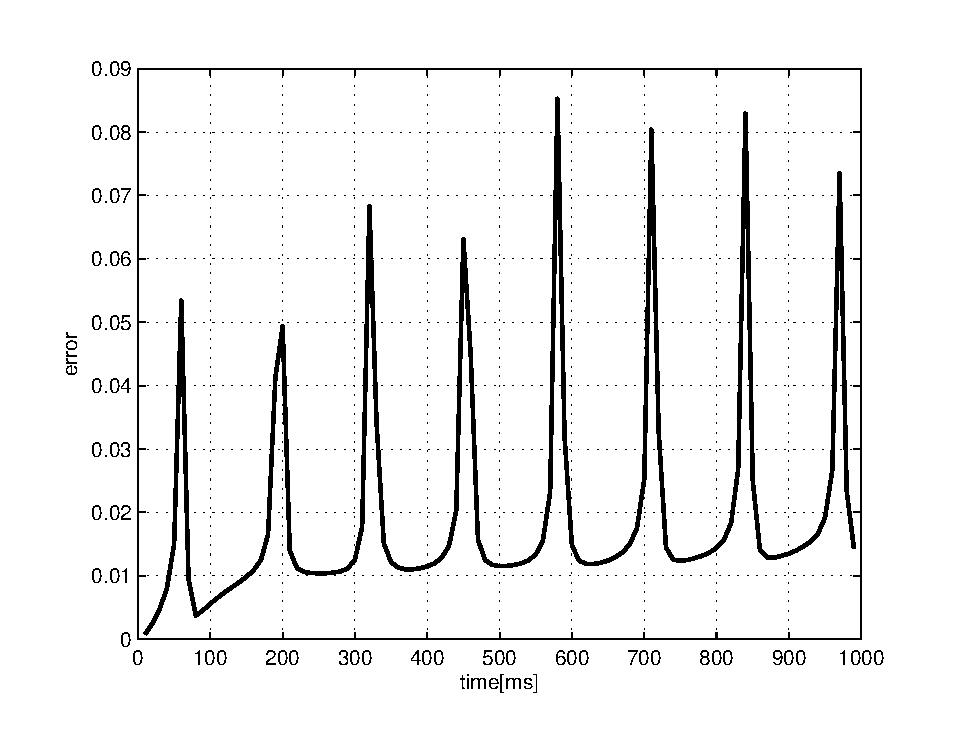
\includegraphics[height = 3.5 cm]{fig/numerical_example_MDE_exp3_error}
\caption{evolution of the error in time.}\label{fig:mde_ex3_error}
\end{figure}
\end{frame}

\begin{frame}
\begin{itemize}
\item Assemble of exact problem: 393.883 [seg]
\item Assemble of homogenized problem: 0.0595 [seg]
\item Total time for exact problem: 1338.2 seg
\item Total time for homogenized problem: 2,089 seg
\end{itemize}
\begin{figure}[H]
\centering
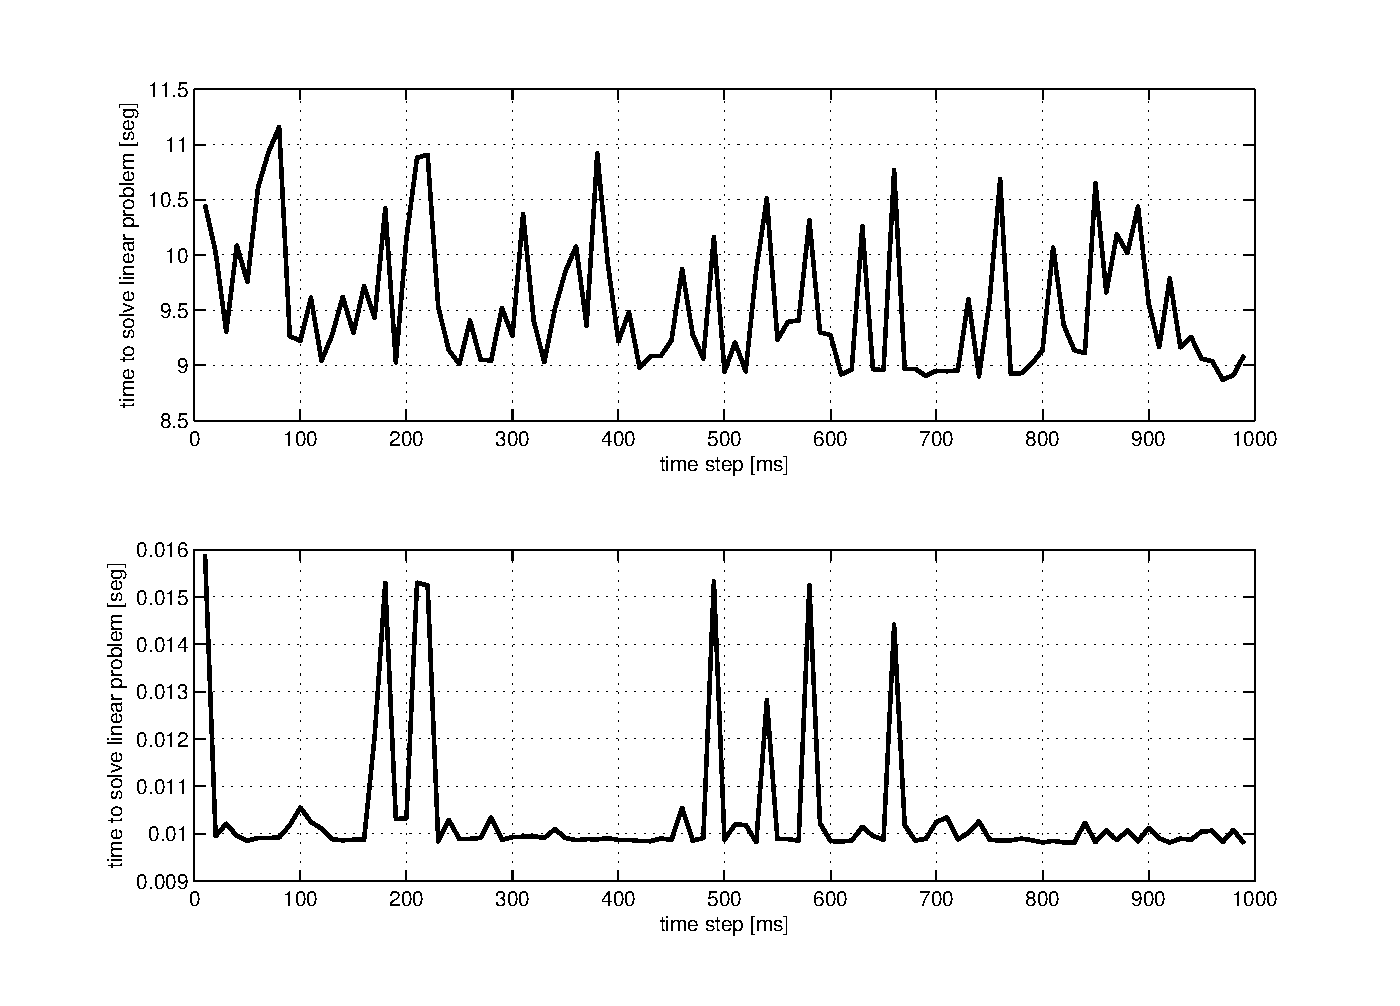
\includegraphics[height = 5 cm]{fig/numerical_example_MDE_exp3_benchmark}
\caption{tiempo de computo para cada paso de tiempo.}
\end{figure}
\end{frame}

\begin{frame}
Algunas Conclusiones:

\begin{itemize}
\item Sobre la Homogeneización:
\begin{itemize}
\item Error tolerable para solución procedente de \textsl{surrogate model}. \pause
\item Bajo costo computacional. \pause
\item Poco sensible a variación de parámetros (incluso para altas fracciones de tejido fibroso). \pause
\end{itemize}
\item Sobre el sistema lineal:
\begin{itemize}
\item Estable \pause $\rightarrow$ $\Delta t = 10 ms$ (máximo) realista para las escalas de tiempo que se manejan.
\item Bajo costo computacional (lineal y desacoplado).
\end{itemize}
\end{itemize}
\end{frame}

\begin{frame}
\begin{center}
\Huge Por Hacer...
\end{center}
\end{frame}

\begin{frame}{To Do}

\begin{itemize}
\item Escalar potencial para obtener ``valores fisiológicos''. \pause
\item Investigar configuración que permite la aparición de ondas en espiral (c. de borde) \cite{TenTusscher2007Europace}. \pause
\item Implementar forma mas realista de considerar áreas con colágeno \cite{Comtois2011IEEE}. \pause
\item Estudiar isotropía del colágeno.
\item Evaluar implementación de otro modelo para la actividad eléctrica de la membrana celular, que incorpore la diferencia de comportamientos entre distintos sectores del corazón. \pause
\item Mallas realistas (3-D). \pause
\item Evaluar implementación de modelo Bi-Dominio. \pause
\item Acoplar modelo electrofisiológico a algún modelo mecánico (como el de elasticidad lineal). \cite{Kirk2014pp}. \pause
\item \red{Postular a postgrado!}
\end{itemize}
\end{frame}


\begin{frame}
\begin{center}
\bibliography{biblio_fibrosis}{}
\bibliographystyle{plain}

\end{center}
\end{frame}

\end{document}	
\end{document}
